\documentclass{article}
\usepackage{hyperref}
\usepackage{graphicx}
\usepackage{pdfpages}

\begin{document}

\title{EngMath - ps\_2}
\author{A. Q. Snyder}
\date{\today}

\maketitle

\section{Problem Set template}

For more details, the entire template and its supplementary materials can be found on GitHub: \href{https://github.com/aqsnyder/eng_math/tree/main/ps_2}{https://github.com/aqsnyder/eng_math/tree/main/ps_2}.
Under the ps\_2 directory exist the necessary files for this LaTeX generation, the compiled plots, and MATLAB exports.
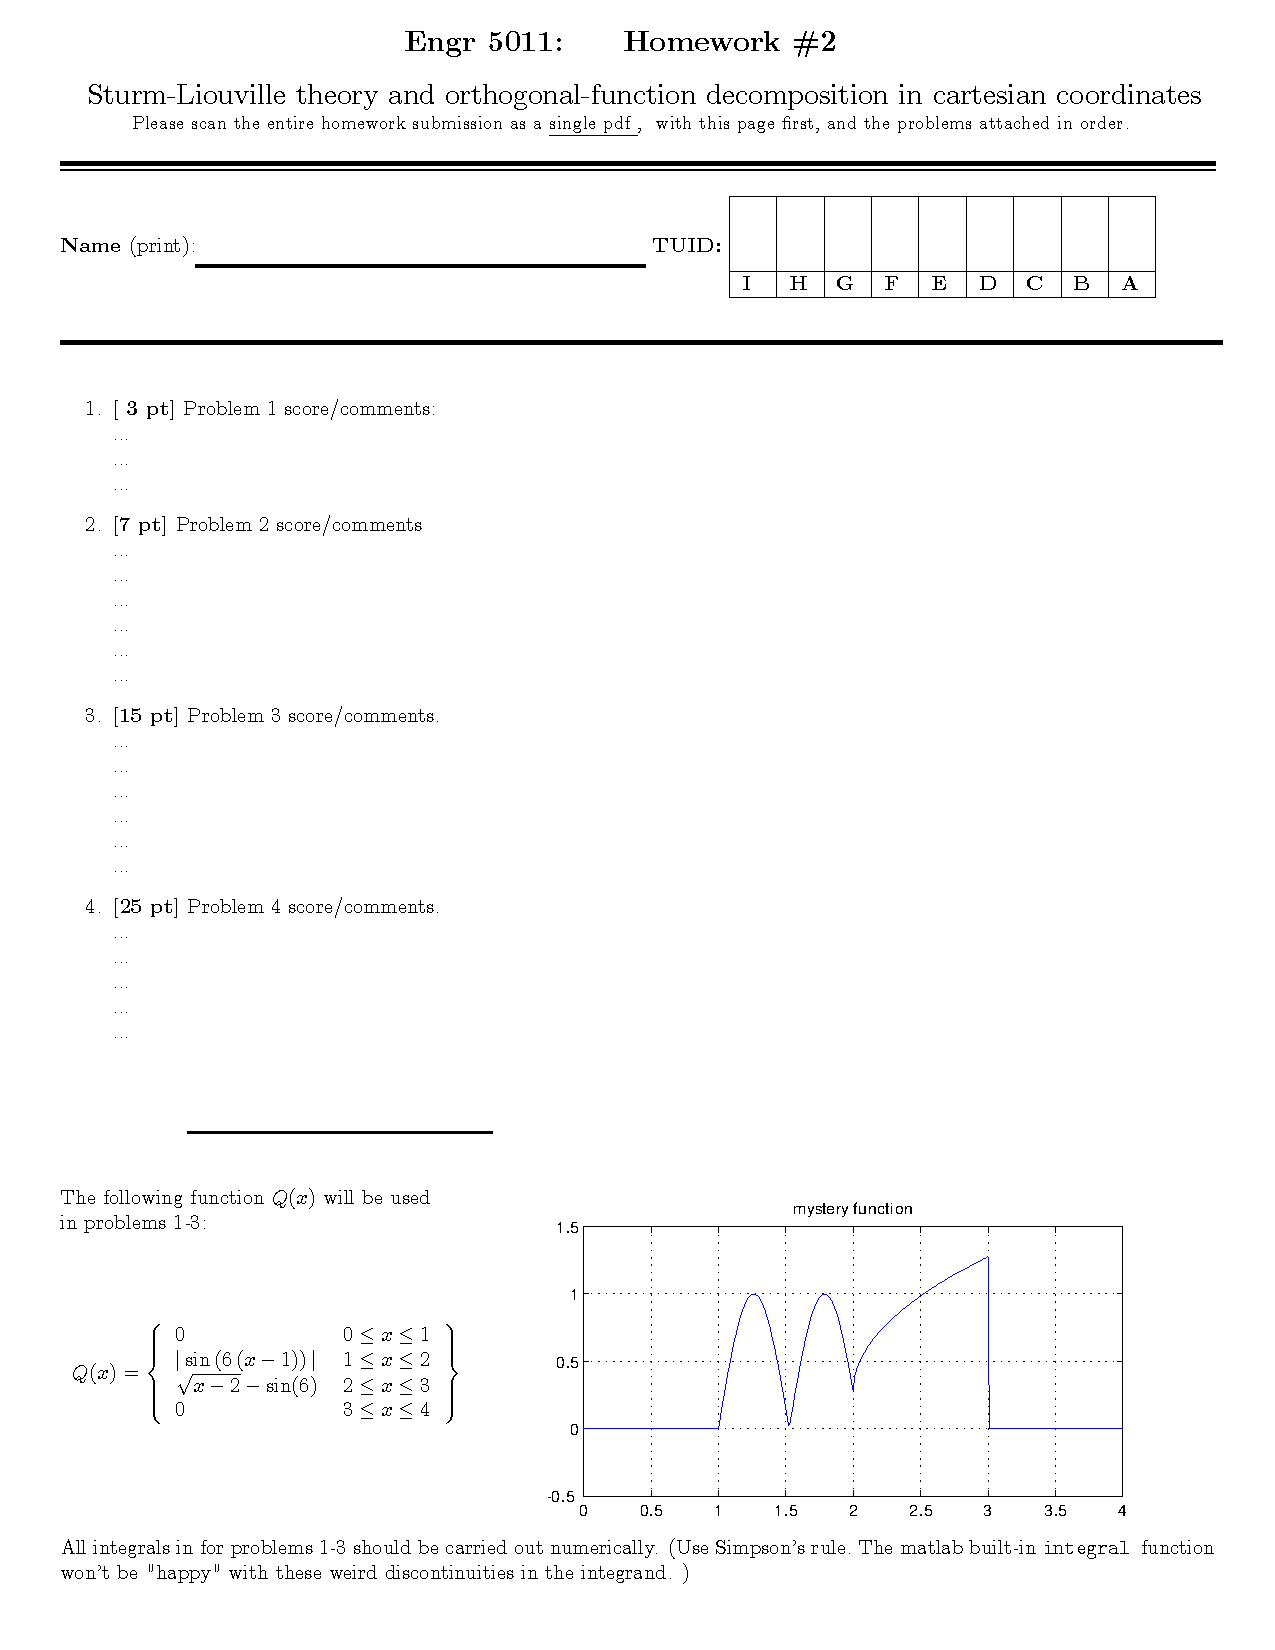
\includepdf[pages=-]{misc_media/hw_2_prompt.pdf}

\section{Hand Calcs}
\vspace{2cm}  % Add vertical space of 2cm

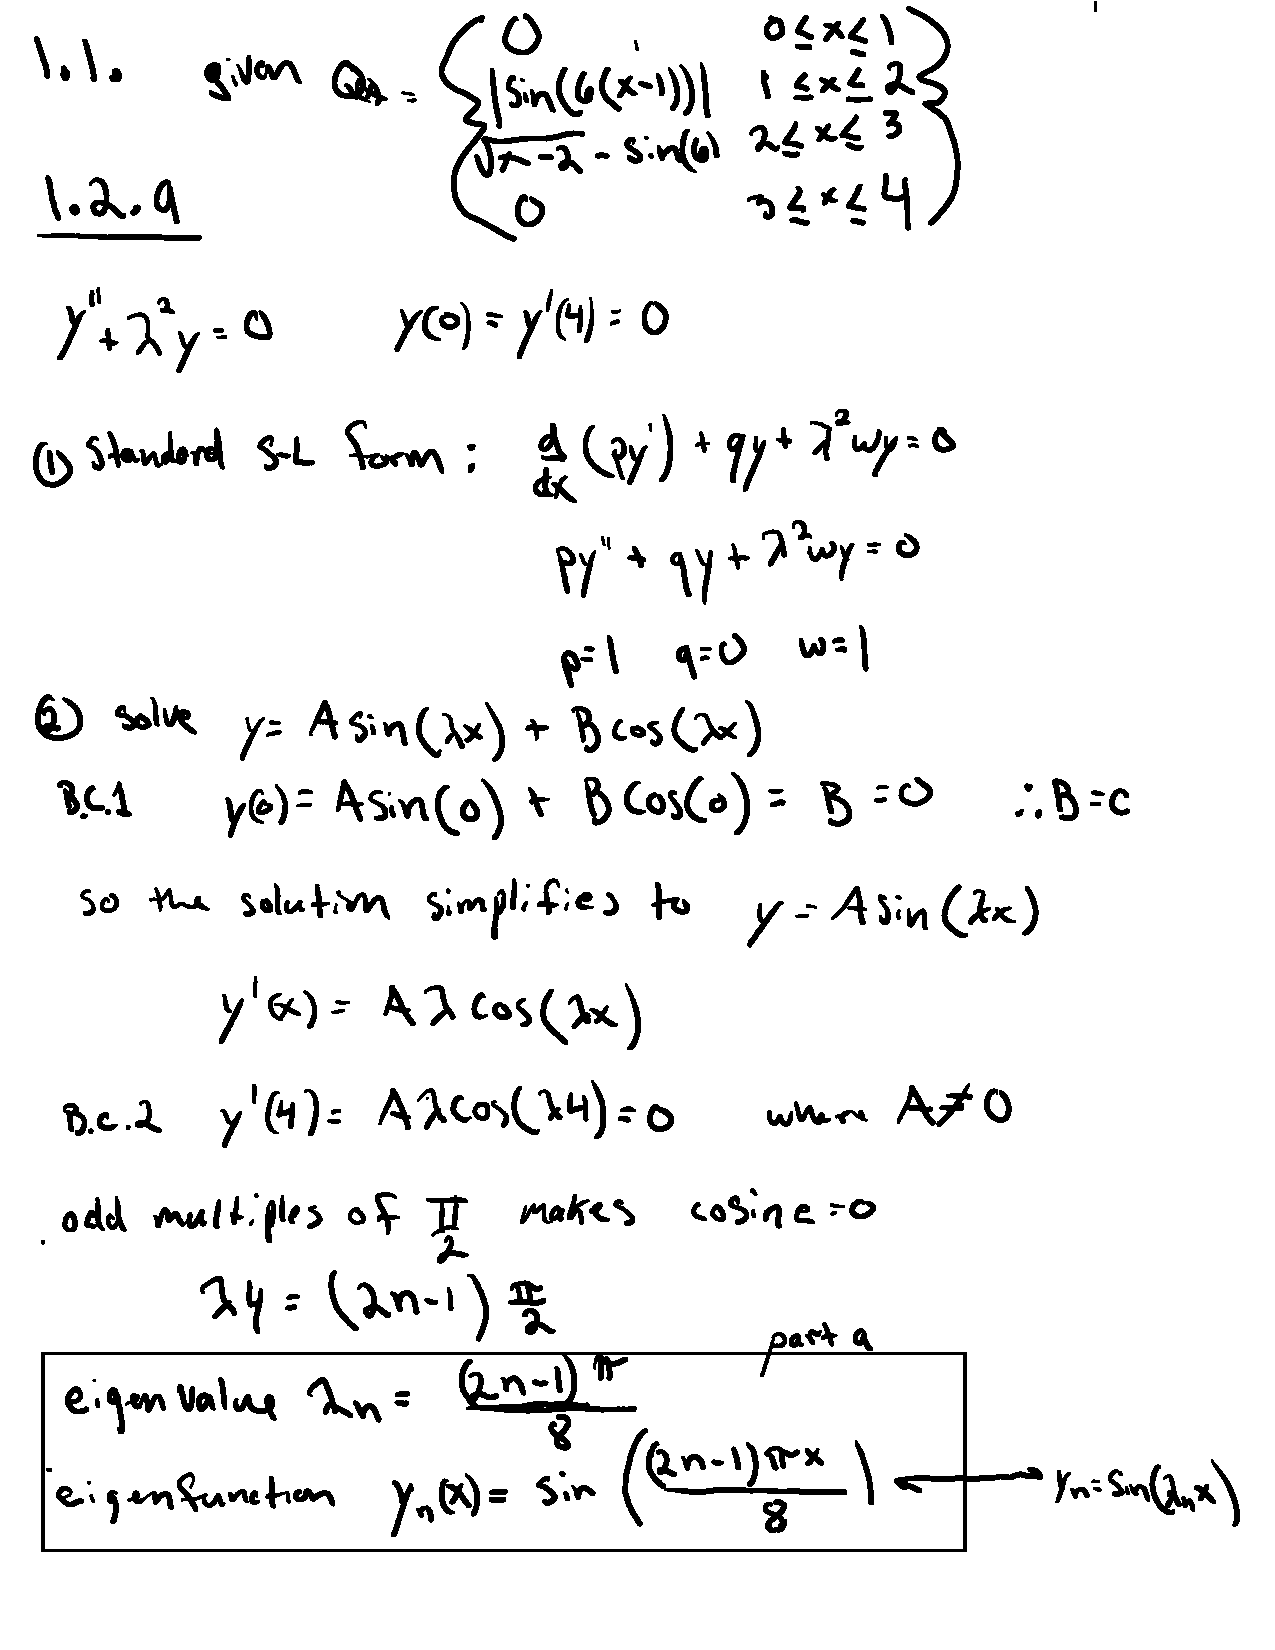
\includepdf[pages=-]{hand_calcs/1.pdf} 
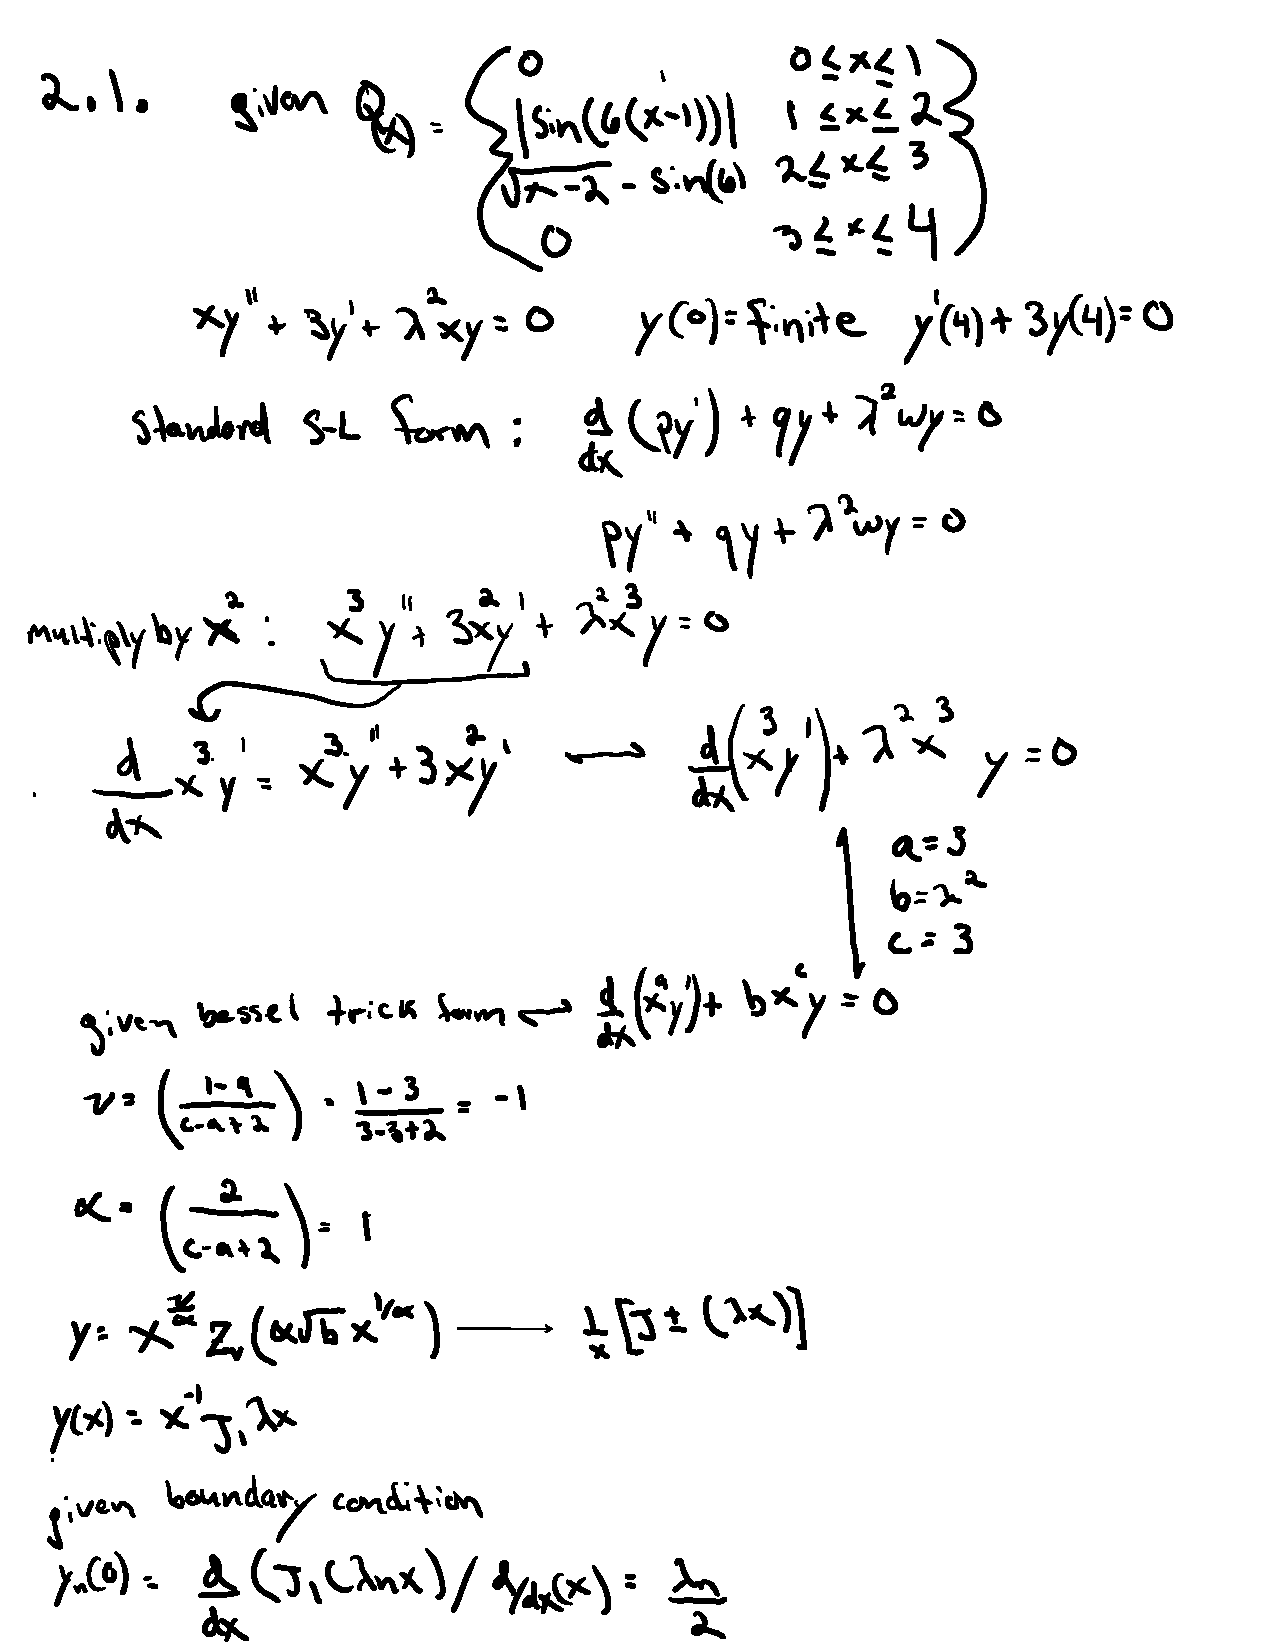
\includepdf[pages=-]{hand_calcs/2.pdf} 
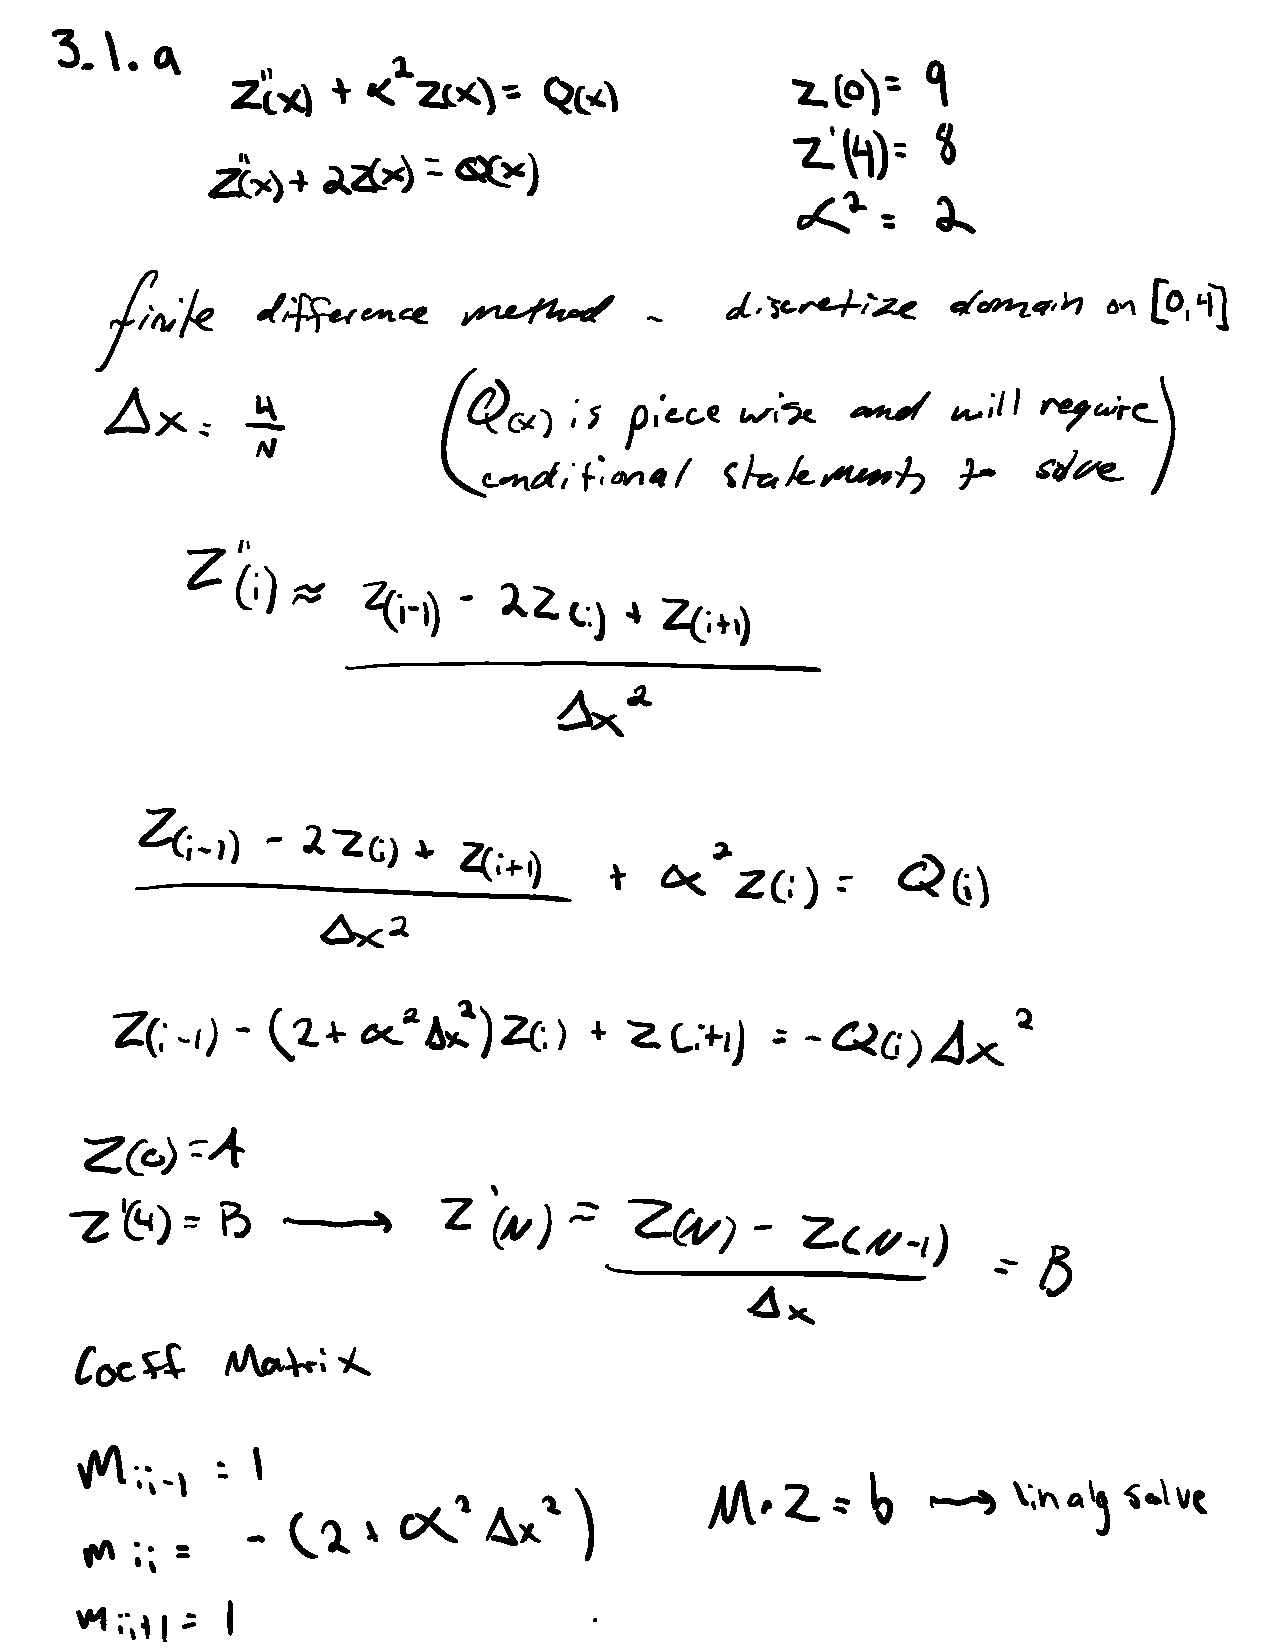
\includepdf[pages=-]{hand_calcs/3.pdf} 
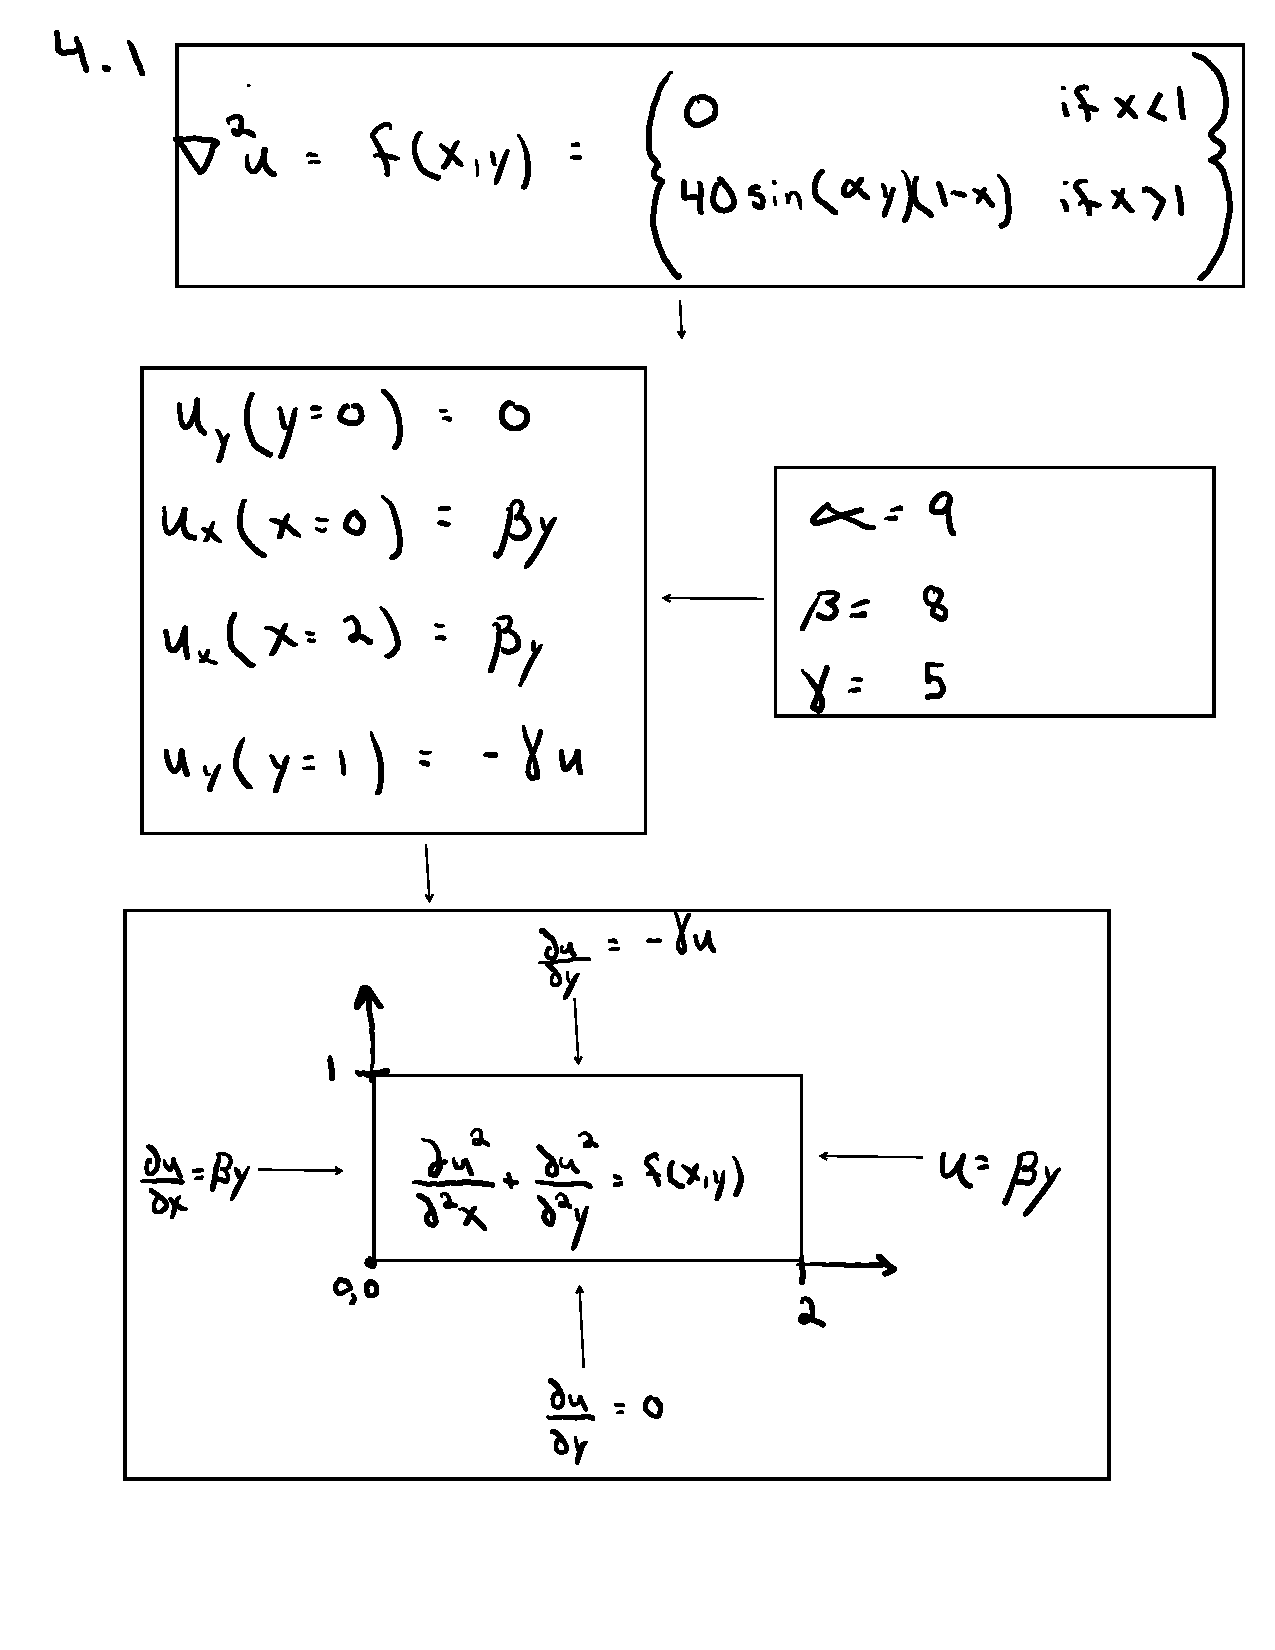
\includepdf[pages=-]{hand_calcs/4.pdf} 

\section{Matlab Outputs}
\vspace{2cm}  % Add vertical space of 2cm

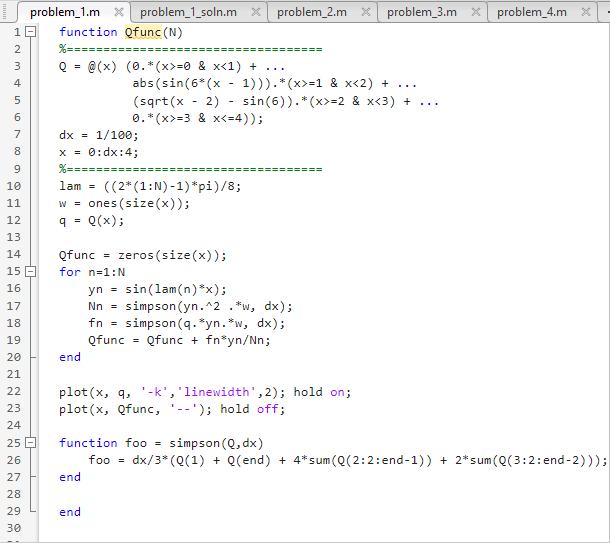
\includepdf[pages=-]{compiled_outputs/matlab_functions/1a.png}
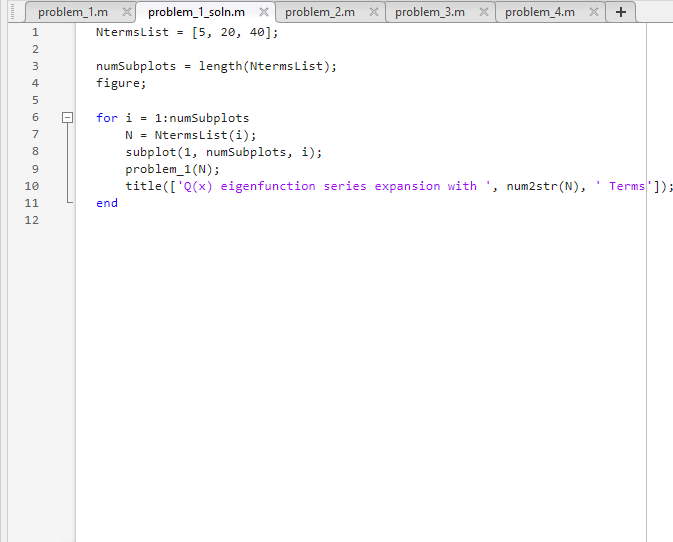
\includepdf[pages=-]{compiled_outputs/matlab_functions/1b.png}
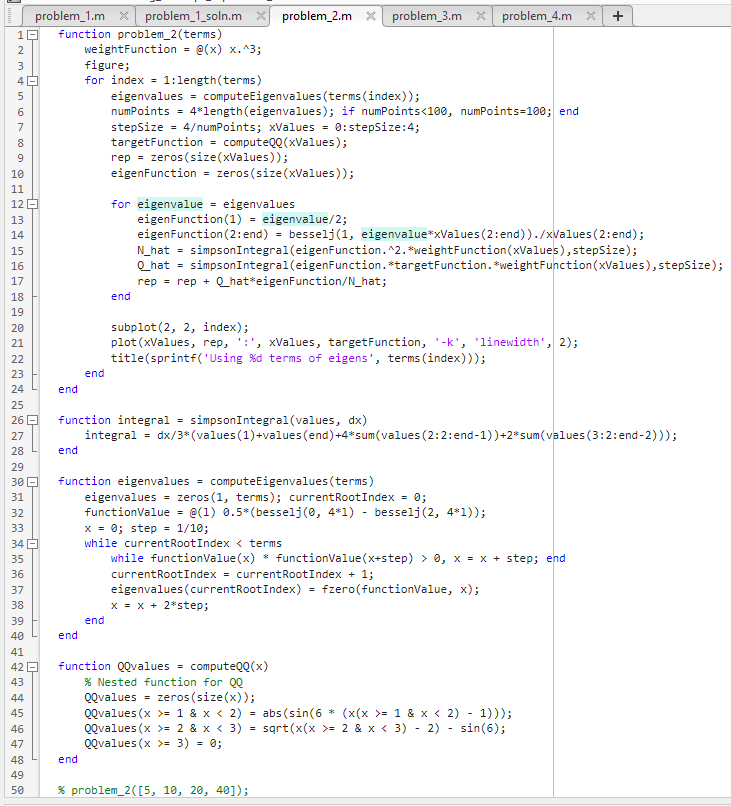
\includepdf[pages=-]{compiled_outputs/matlab_functions/2.png}
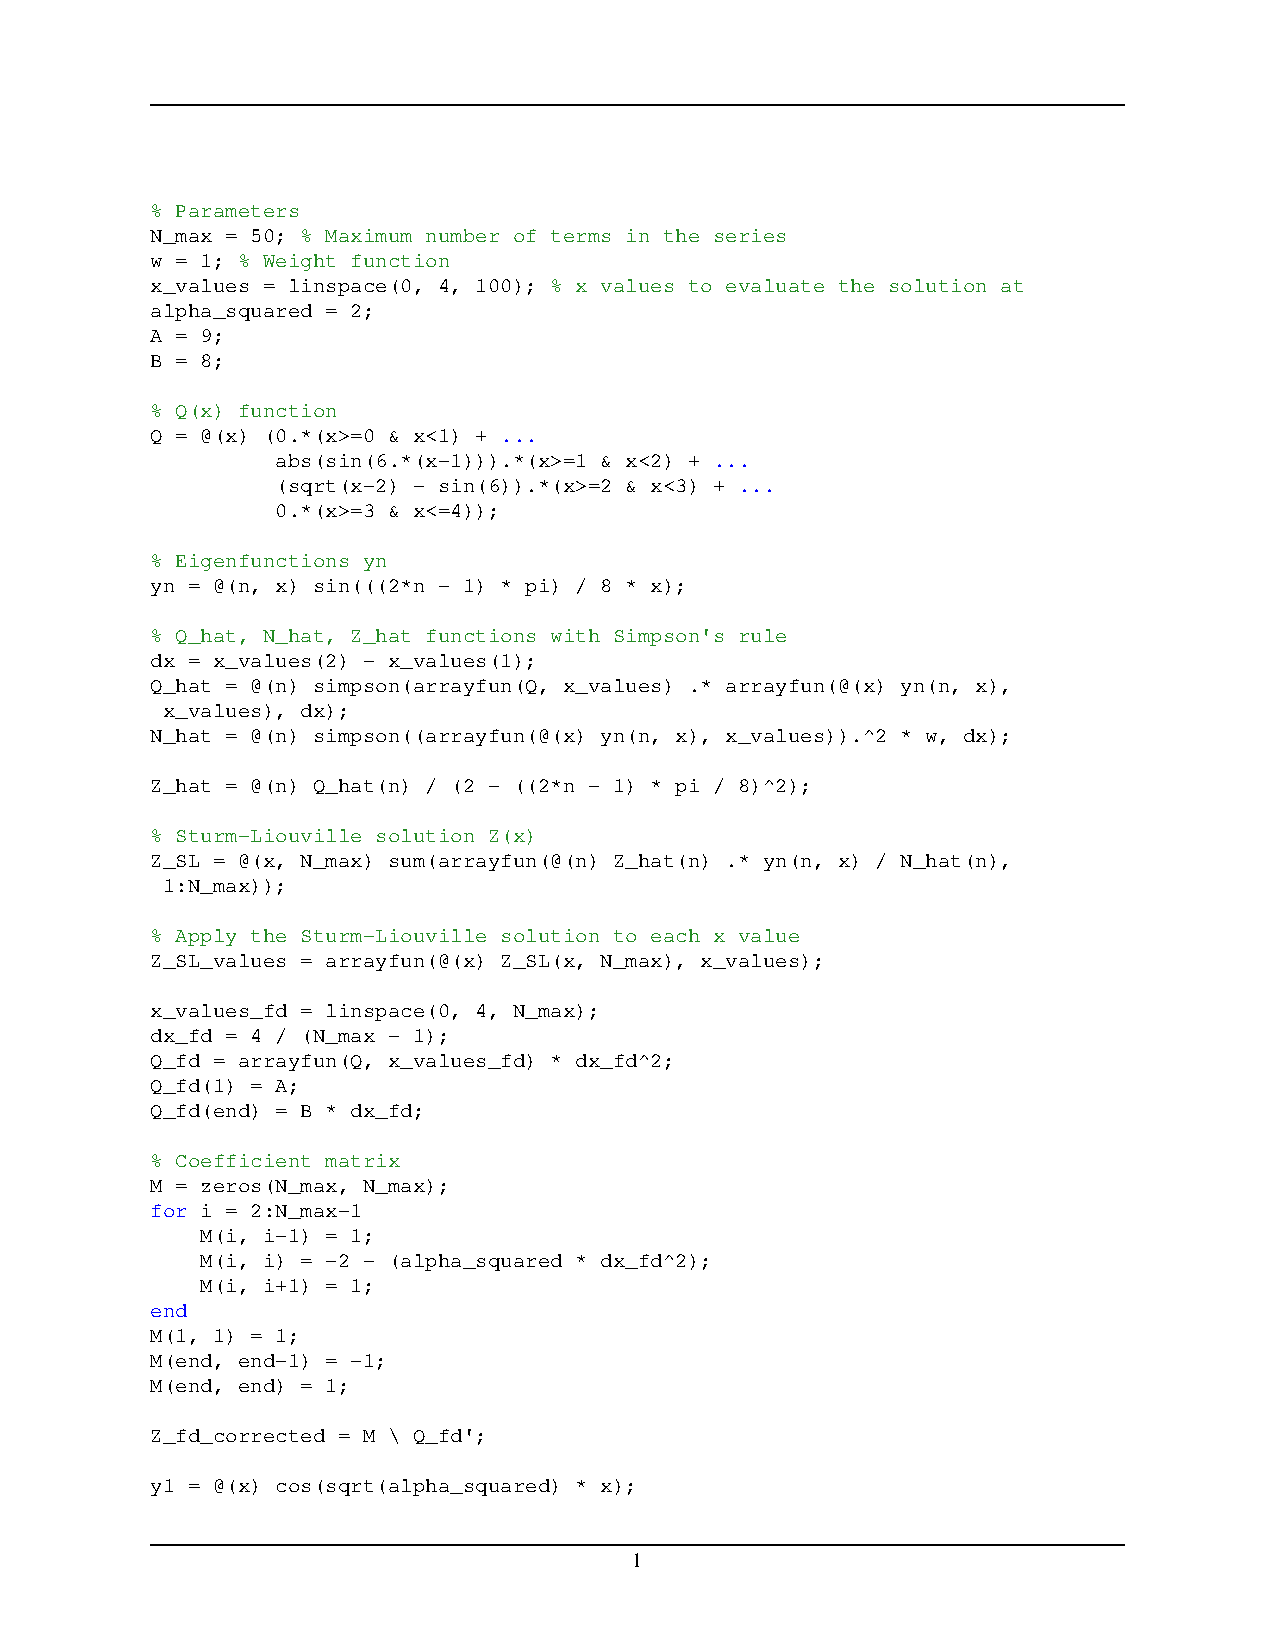
\includepdf[pages=-]{compiled_outputs/matlab_functions/3.pdf}
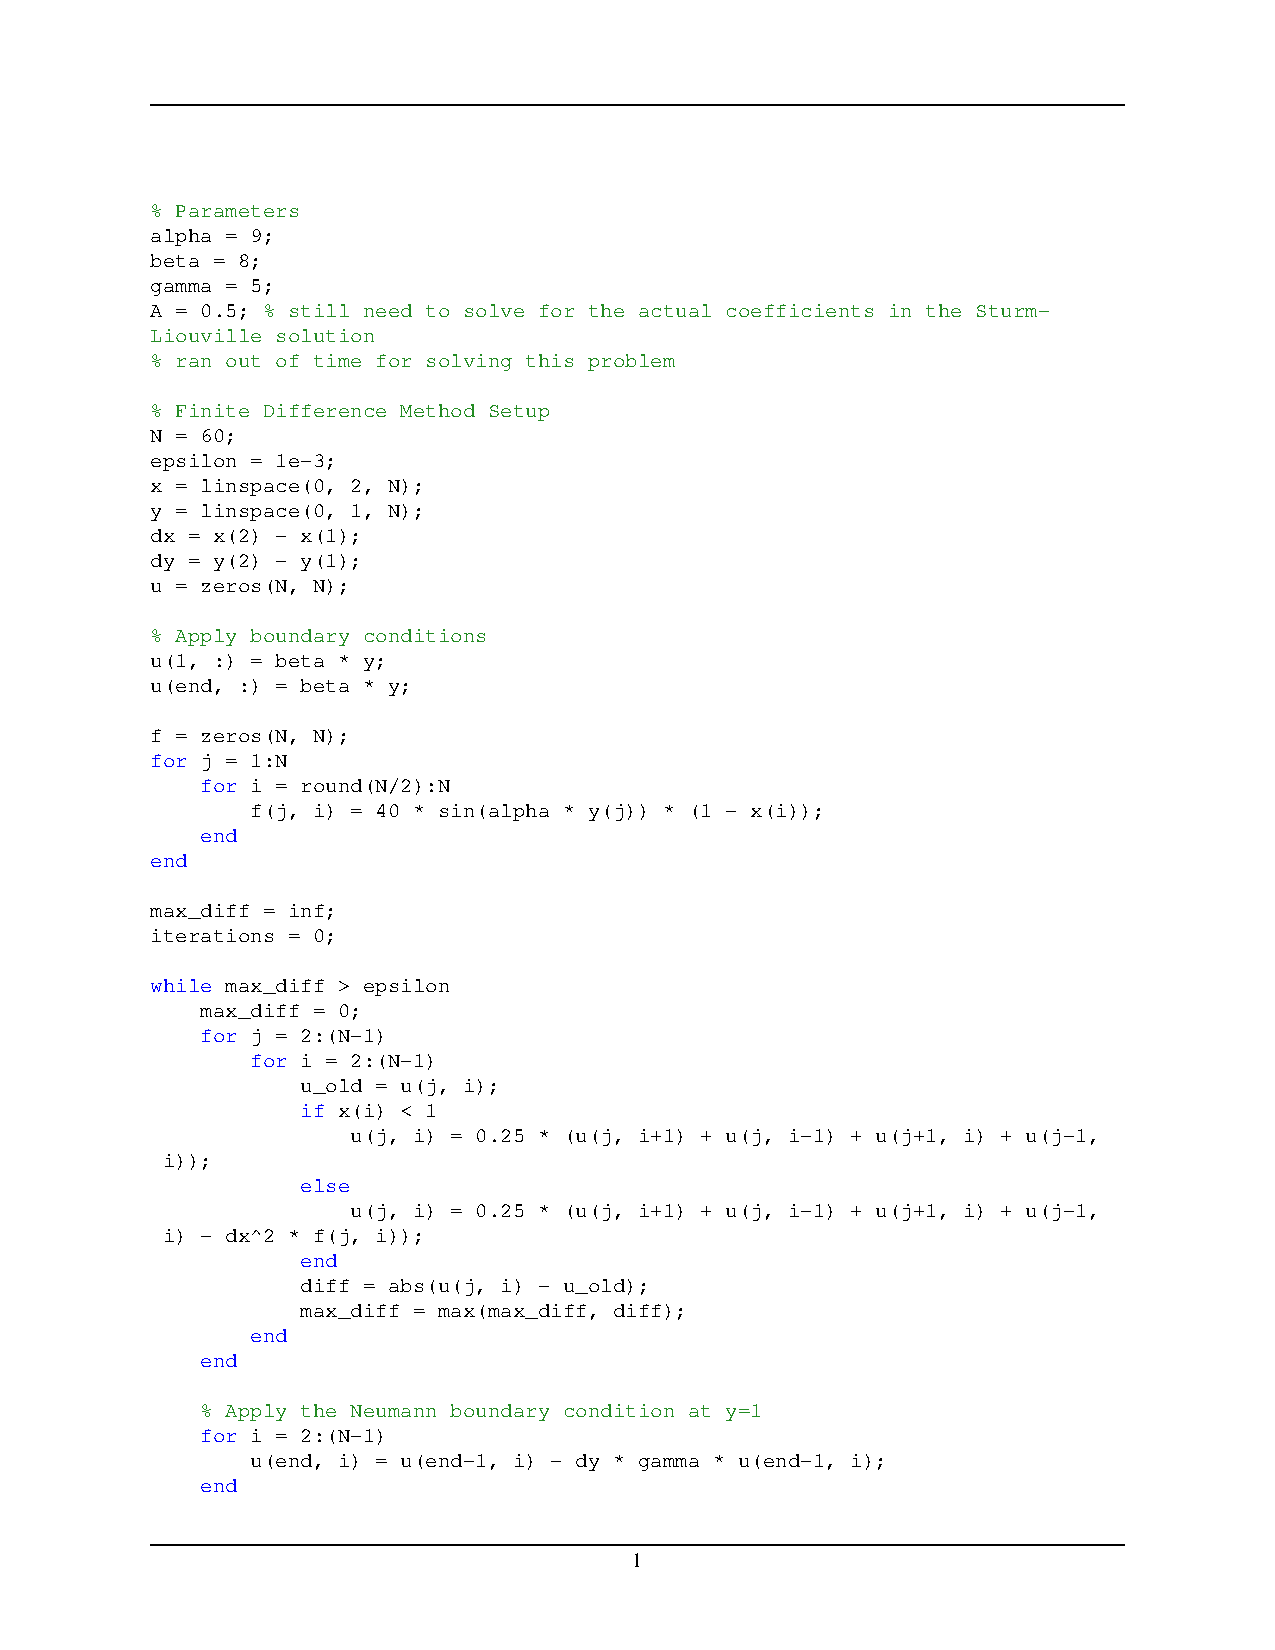
\includepdf[pages=-]{compiled_outputs/matlab_functions/4.pdf}

\section{Compiled Plots}
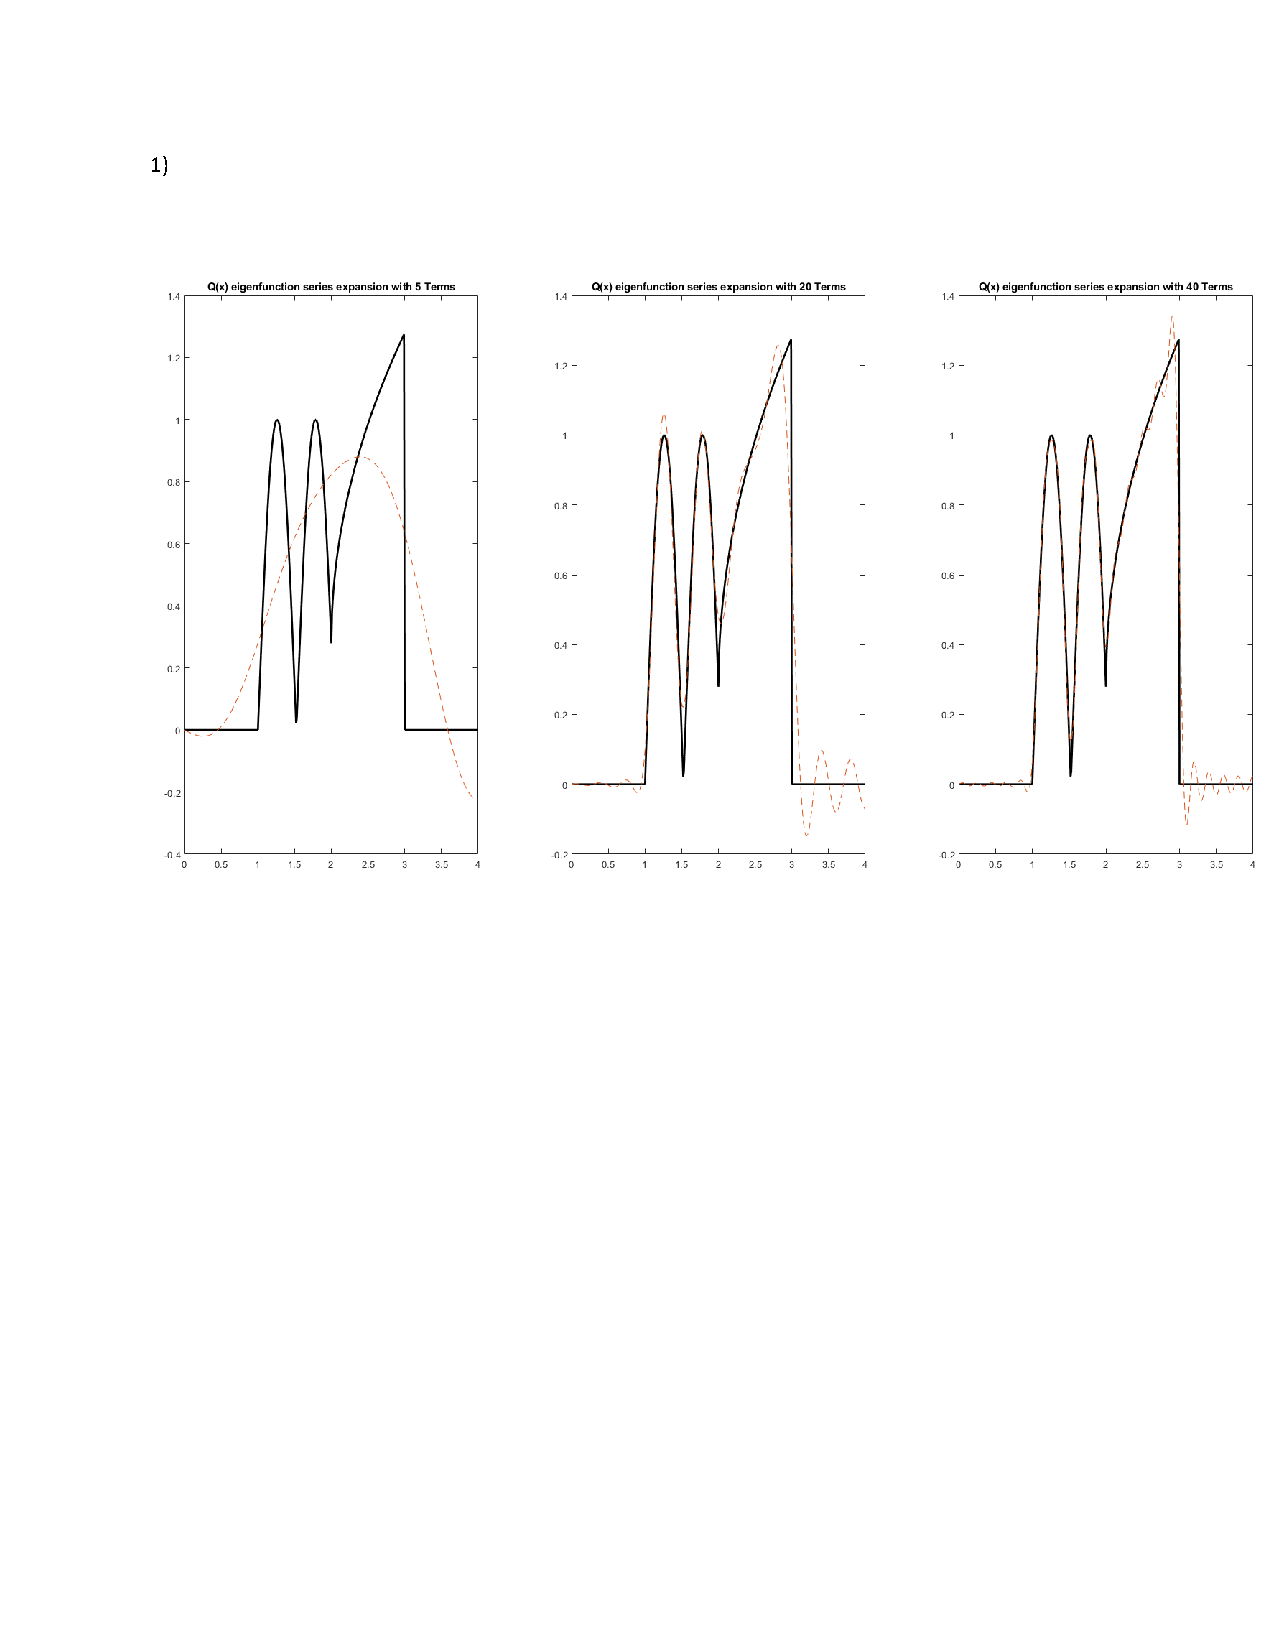
\includepdf[pages=-]{compiled_outputs/compiled_plots.pdf}

\end{document}
